Previous literature utilized gasses such as \ce{NO}, \ce{CH4}, \ce{N2O}, and \ce{Kr} to separate the isomers.\todo{citations} \ce{Kr}, and \ce{Xe} are inert and would not react with any other trapped ion but are too heavy to reliably trap after a reaction. \ce{NO} is caustic and will ruin the vacuum chamber if introduced, and thus was avoided. Attempts were make with \ce{N2O} and well as \ce{CH4}, but both had their own unique complications. \ce{N2O} rapidly reacts with \ce{Be+} and made reliable TOF traces unattainable due to the loss of the coolant ion. \ce{CH4} readily reacted with most of the ions in the trap to produce a multitude of mass peaks, greatly complicating the analysis.

Normally \ce{N2} would not be a good choice, due to the fact that \ce{N2H+} has the same mass as the formyl isomers at $m/z=29$, but we may instead introduce \ce{^{15}N2} to produce a new peak at $m/z=31$.

We do not expect and do not see any reaction between the initially loaded ions of \ce{Be+} and \ce{C+}. But according to \cref{tab: affinities}, we should still have a separation of the isomers, thus:

\begin{align}
	\ce{Be+ + ^15N2 & -> no reaction} \\
	\ce{C+ + ^15N2 & -> no reaction} \\
	\ce{HCO+ + ^15N2 & -> no reaction} \label{r: HCO+N2->NA} \\
	\ce{HOC+ + ^15N2 & -> ^15N2H+ + CO} \label{r: HOC+N2->N2H}
\end{align}

Considering reactions \ref{r: X+HOC->HCO} and \ref{r: X+HOC->XH}, if we let \ce{X = CO}, we find that both reactions can only yield \ce{HCO+}, allowing us to deterministically produce one of the isomers:

\begin{equation}
	\ce{HOC+ + CO -> HCO+ + CO} \label{r: HOC+CO->HCO}
\end{equation}

To verify reaction \ref{r: HOC+CO->HCO}, trapped \ce{Be+} and \ce{C+} ions are exposed to the water from the CBGB at a density of $4.3 \times 10^6$ cm$^{-3}$ while simultaneously flooded with $\approx 3 \times 10^7$ cm$^{-3}$ of \ce{CO} from the leak valve connected to the differential pumping region such that $k_{\ref{r: HOC+CO->HCO}} \gg k_{\ref{r: C+H2O->HCO}, \ref{r: C+H2O->HOC}}$. After 10 s, the gate valve between the differential pumping and experimental ion chamber regions is manually closed, after which, $10^9$ cm$^{-3}$ of \ce{^15N2} is introduced for 10 s. A TOF trace for this procedure is shown in figure \ref{fig: CO N2 TOF}.

\begin{figure}[H]
	\centering
	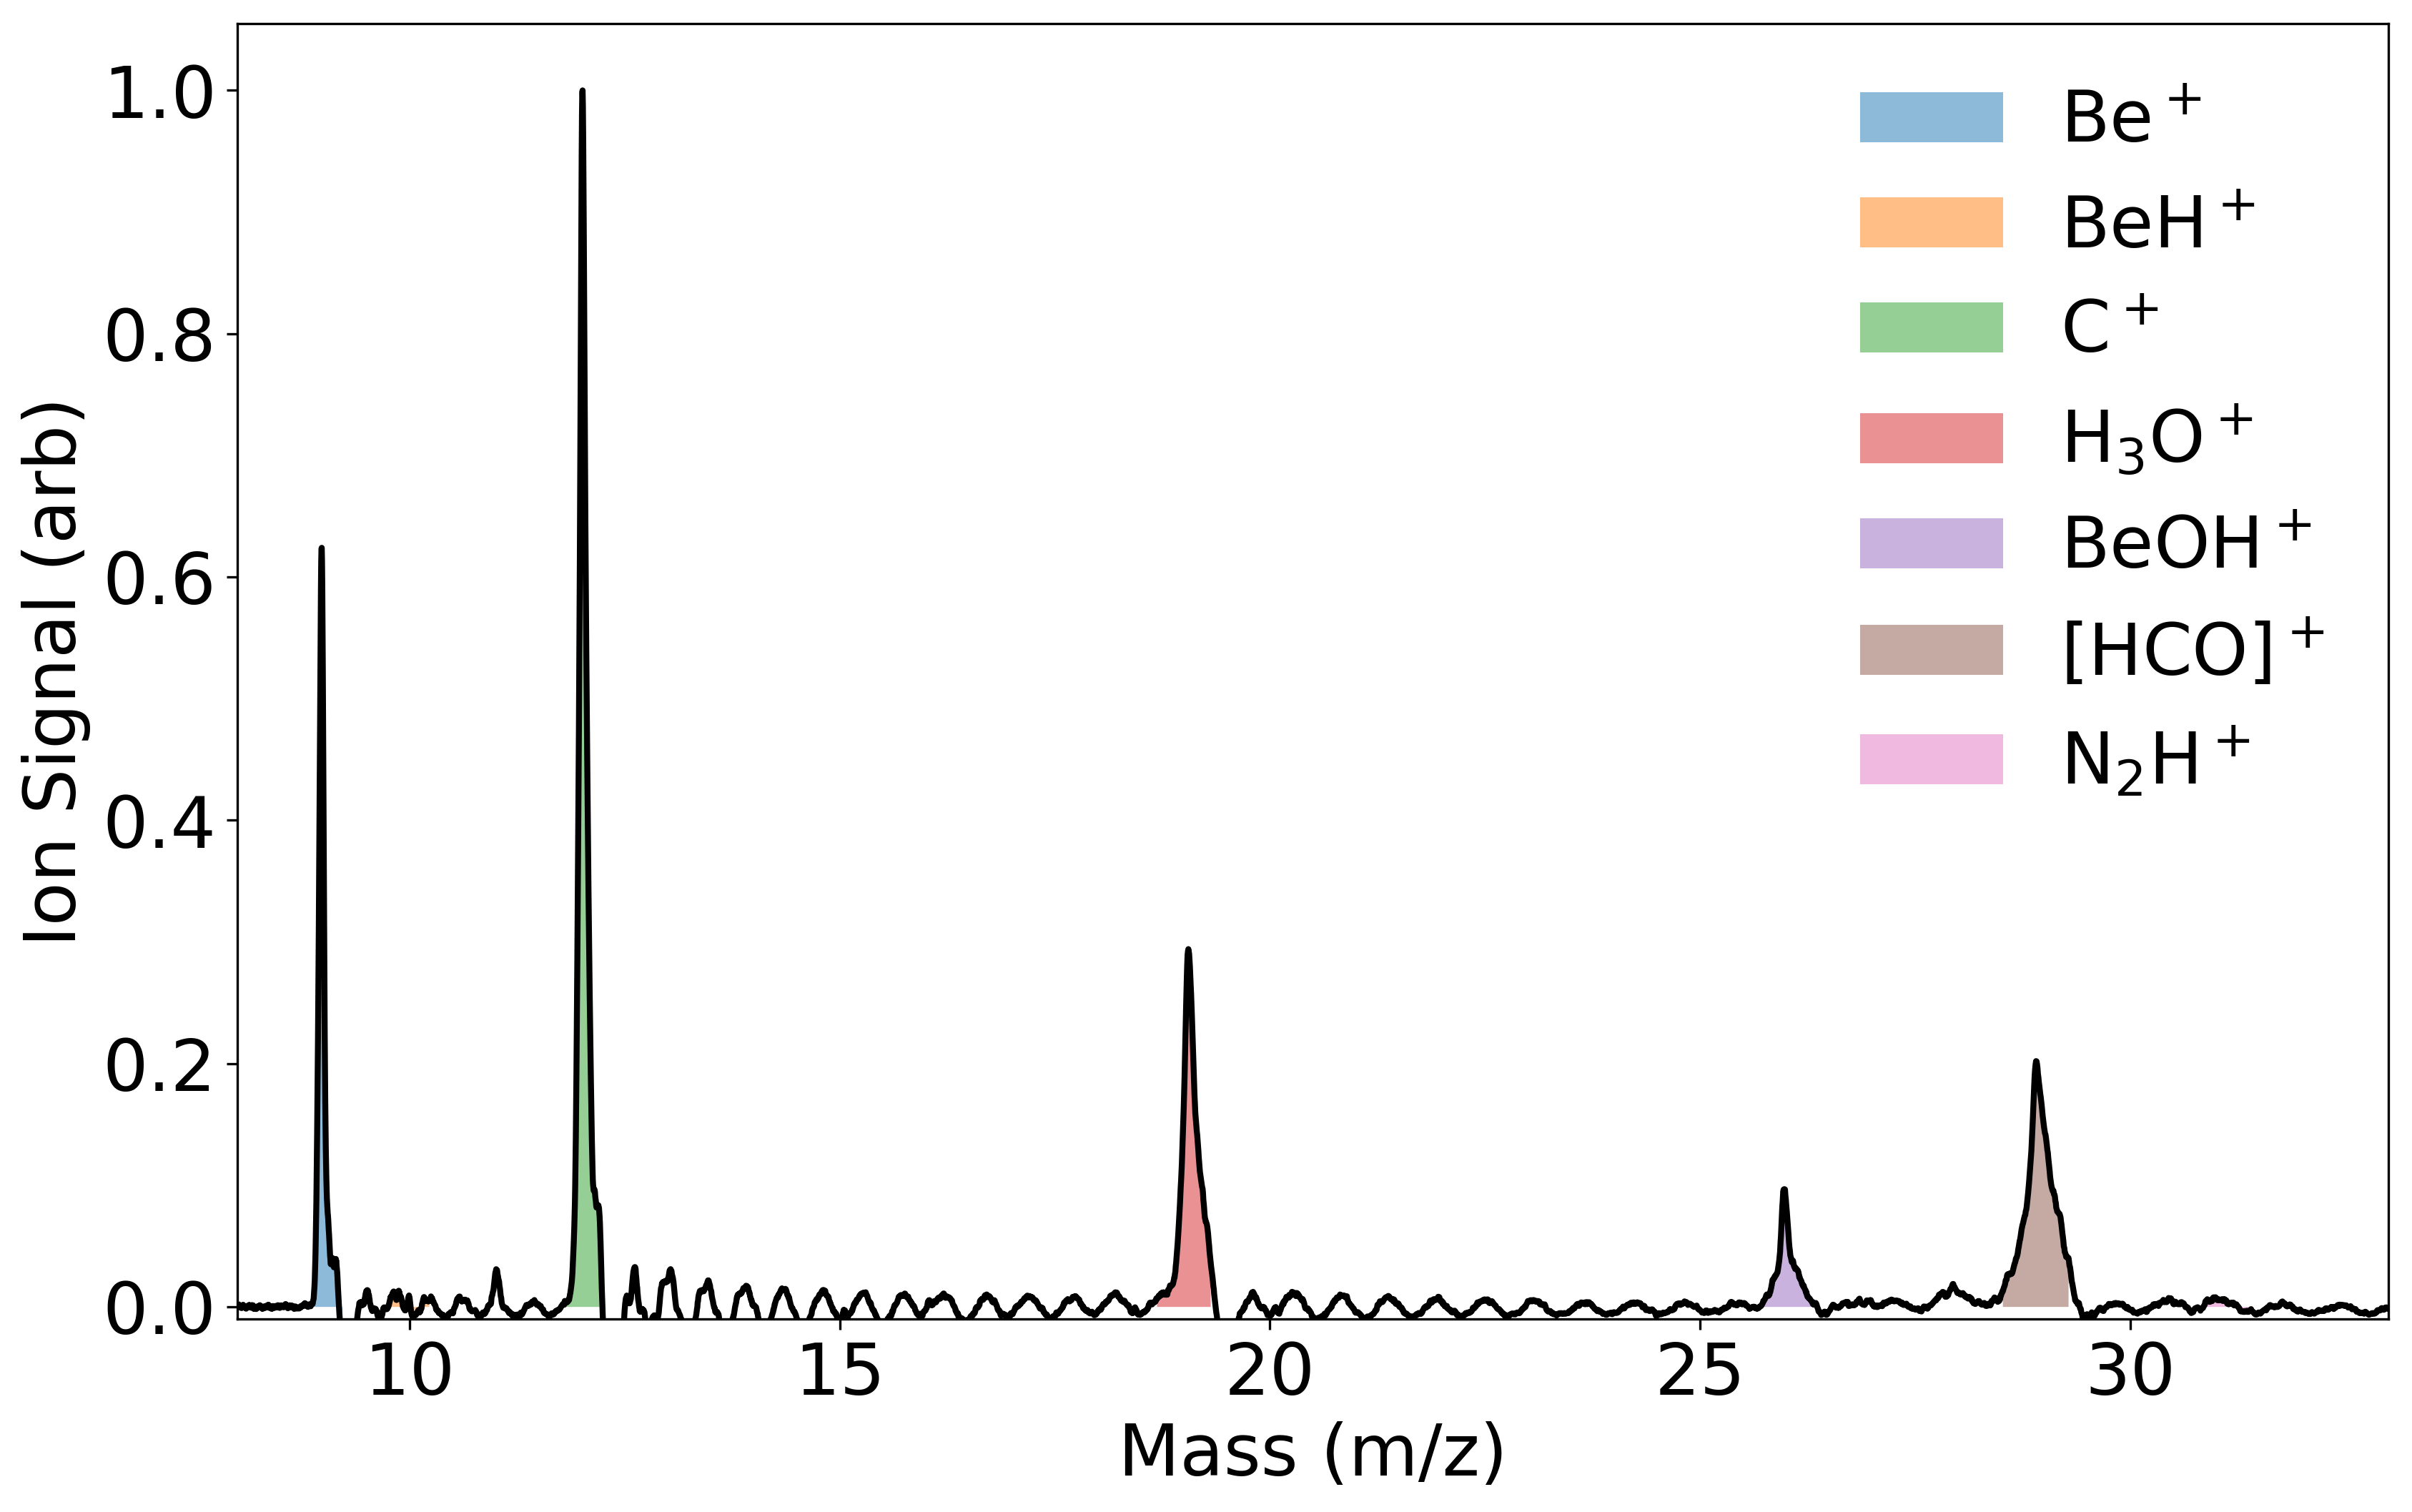
\includegraphics[width=0.8\textwidth]{images/C_H2O_CO_15N2.png}
	\caption{TOF trace of reaction products of \ce{Be+} and \ce{C+} after exposure to both water from the CBGB beam, and \ce{CO} (10 s) before titration with \ce{15N2} (10 s). There is a distinct lack of \ce{N2H+}, indicating full conversion of \ce{HOC+ -> HCO+}.}
	\label{fig: CO N2 TOF}
\end{figure}

Integrated \ce{N2H+} signal was found to be below the threshold for null signal demonstrating both points that reaction \ref{r: HOC+CO->HCO} proceeds as expected, as well as experimental verification that reaction \ref{r: HCO+N2->NA} does not occur. Extending this process, we consider the possibility that reactions \ref{r: HCO+H2O->H3O} and \ref{r: HOC+H2O->H3O} are different by again exposing \ce{C+} to \ce{H2O} from the beam to produce \ce{[HCO]+}, eliminating the \ce{HOC+} with \ce{CO}, and finally exposing the everything to \ce{H2O} again. \todo{verify rate constants}

\begin{figure}[H]
	\centering
	\missingfigure{blah}
	\caption{text}
	\label{fig: [HCO] rate}
\end{figure}